\section{Déroulement du projet}

\subsection{Systemtap}

\subsubsection{Principe de fonctionnement}

Nous avons ainsi commencé par utiliser Systemtap, un outil d'analyse du noyau grâce à des scripts qui ne nécessitent pas de modifier le code du noyau. Systemtap utilise les KProbes, et les Kretprobes\cite{IBMRBST} pour intervenir à différents endroits dans le déroulement des fonctions du noyau pour permettre à l'utilisateur de lire certaines variables ou de logger certains appels système. Le principe de fonctionnement de Systemtap est résumé sur le schéma ci-dessous.

\begin{figure}[hb]
	\centering
	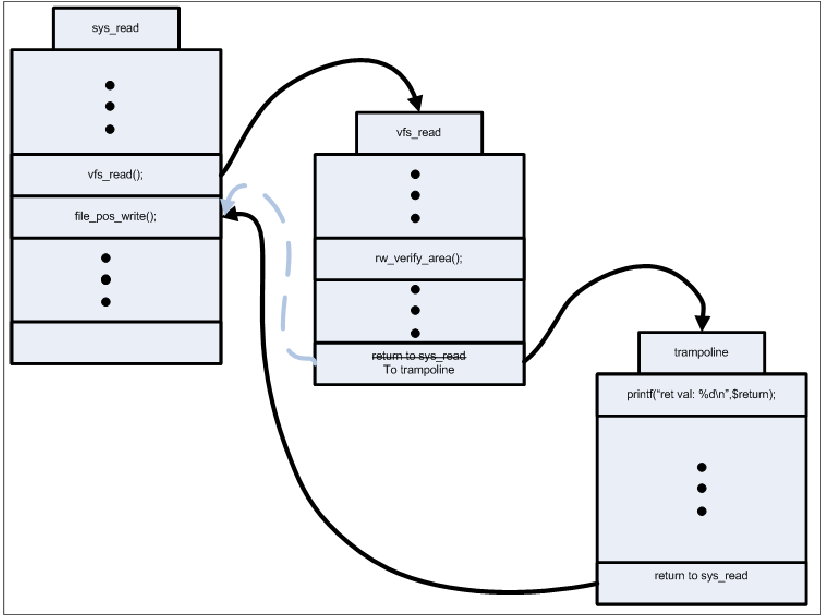
\includegraphics[scale=0.4]{kretprob.png}
	\caption{Fonctionnement tel que décrit dans la référence IBM sur Systemtap \cite{IBMRBST}}
\end{figure}

\subsubsection{Résultats obtenus}

Après s'être familiarisé avec le fonctionnement de Systemtap, nous nous sommes aperçu que les scripts utilisés pour récupérer les informations issues des appels système sont exécutés une fois l'appel système effectué. Il n'est pas possible, d'après nos recherches, de faire en sorte que les scripts puissent bloquer les appels système avant de les effectuer.

De ce fait, l'utilisation de Systemtap ne permet pas de répondre à nos besoins.

Il faut ajouter à cela que les informations recueillies à partir de Systemtap ne sont pas exploitables pour certaines d'entre-elles. Par exemple, lorsqu'un fichier est accédé (lu ou écrit), seul le numéro d'inode nous était retourné. Il n'était alors pas pertinent de récupérer le chemin complet du fichier, car cette recherche est inadaptée et inefficace : il est nécessaire de parcourir l'intégralité du système de fichiers.

Il fallait donc changer de stratégie. C'est pourquoi, nous avons, avec l'accord du responsable du projet, décidé de nous orienter vers l'utilisation des ``Linux Security Modules'' (LSM).

\subsection{Linux Security Modules}

\subsubsection{Principe de fonctionnement}

Les modules LSM sont au noyau ce que netfilter est au réseau.

Le principe de fonctionnement est simple : un module LSM est chargé dans le noyau Linux au démarrage. Il se substitue ou complète alors la procédure de contrôle d'accès. \`A chaque appel système est associé un hook que l'on peut considérer comme une fonction. Il est placé dans l'appel système entre les vérifications élémentaires (existence des fichiers, droits unix) et sa réalisation. Dès qu'un appel système est demandé, le hook est exécuté. Par défaut, il autorise l'exécution de l'appel système.

\begin{figure}[hb]
	\centering
	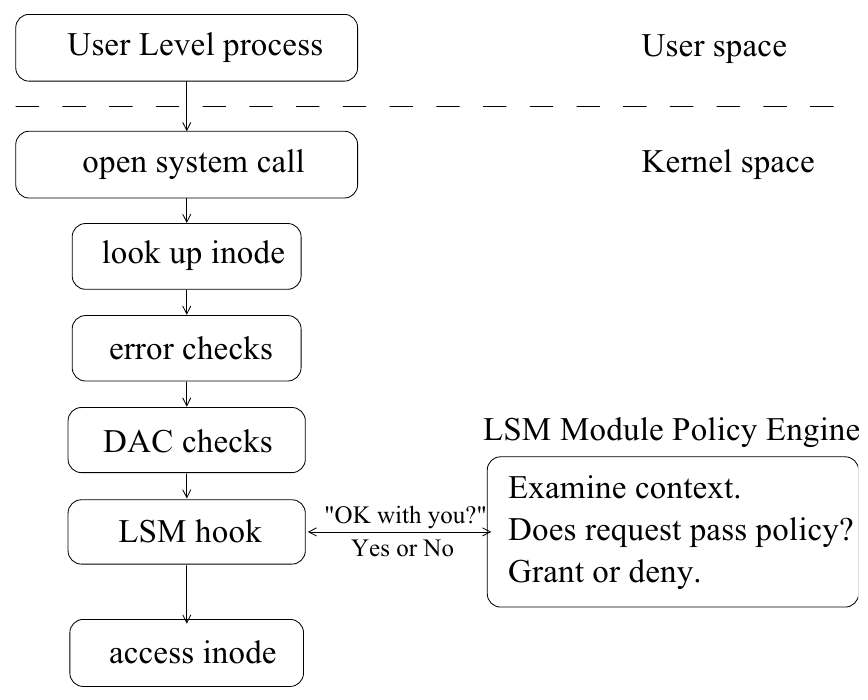
\includegraphics[scale=0.45]{lsm1.png}
	\caption{Architecture des hooks LSM \cite{LSMINTRO}}
\end{figure}

L'avantage de ces hooks est qu'ils offrent une très grande liberté. Cependant, il n'est possible pour le moment de ne charger dans le noyau qu'un seul et unique module LSM. Or, PIGA-OS utilise déjà un module LSM : SELinux.

\begin{figure}%[hb]
	\centering
	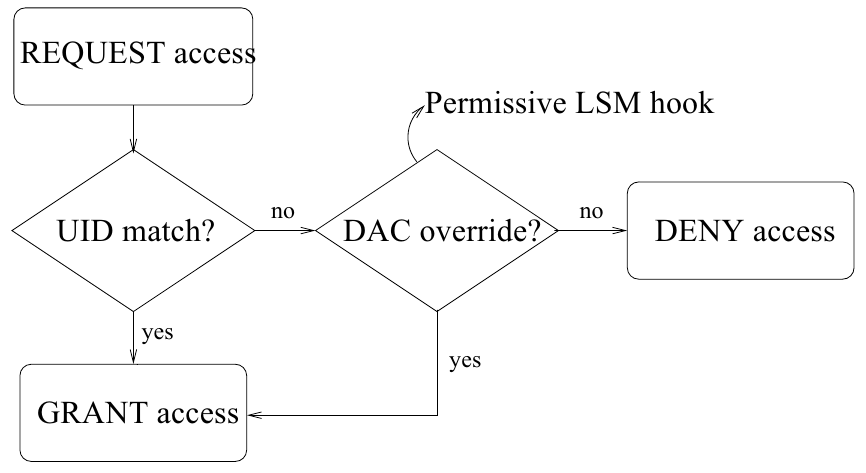
\includegraphics[scale=0.45]{lsm2.png}
	\caption{Hook LSM permissif. Ce hook autorise la politique de sécurité à passer outre les restrictions DAC \cite{LSMINTRO}}
\end{figure}

Pour les besoins du développement, nous avons dû désactiver SELinux, pour nous concentrer sur notre propre module, et non sur l'intégration avec le module LSM de SELinux.

\subsubsection{Implémentation}

Nous avons donc développé un module LSM qui "hook" les appels système. Par défaut, ces hooks sont "transparents" à l'exception du hook "file permission" sur lequel nous avons travaillé. Il est appelé à chaque ouverture (lecture, écriture, exécution) de descripteur de fichier.

Nous avons ajouté la possibilité d'activer ou non ce module lors de la compilation du noyau en suivant les conventions de nommage des options de configuration.

Ensuite, nous avons commencé à chercher les différentes informations nécessaires à contextd pour son fonctionnement, et plus particulièrement ce qui concerne les hooks ``file permission'' et ``mkdir'' :
	\begin{itemize}
		\item le PID
		\item l'execname
		\item le chemin complet du fichier~\\
	\end{itemize}

Nous avons également remarqué que les hooks ``socket\_bind'' et ``socket\_connect'' permetent de récupérer des informations, notamment l'adresse IP et le port de destination d'une socket, avant qu'elle ne soit créée. Ils permettent ainsi d'obtenir l'adresse IP et le port qui correspondent à une connexion. Il existe également deux autres "hooks" ``socket\_recvmsg'' et ``socket\_sendmsg'' qui permettent, eux, de pouvoir exercer un contrôle en fonction du contenu du paquet. On peut donc imaginer grâce à ces quatre "hook" pouvoir surveiller les connexions réseau.

Par manque de temps, nous avons décidé de ne pas surveiller ces "hooks". Cependant, nous avons tout mis en œuvre afin que les informations disponibles dans ces "hook" arrivent à contextd, afin, de pouvoir travailler sur l'exploitation des données et effectuer les contrôls voulus.

En effet, contextd ne permet pas de prendre de décisions sur les adresses IP mais seulement sur les URLs. Une requête DNS inverse ne permet malheuresement pas d'obtenir d'adresse utilisable par contextd. Nous n'avons donc pas poursuivit l'intégration des ``connexions'' dans notre solution.


La principale difficulté de cette étape fut de localiser dans quels fichiers ses informations sont localisées dans l'ensemble du code source du noyau Linux.

\subsection{La communication entre contextd et le noyau}

\subsubsection{Les appels systèmes}

Pour faciliter la communication entre l'espace noyau et le démon en espace utilisateur contextd, nous avons implémenté trois nouveaux appels systèmes. En effet, la solution des appels systèmes nous permet de contrôler les intéractions avec le noyau en créant :
\begin{itemize}
 \item un appel système qui démarre/termine la communication et enregistre/désinscrit les programmes à surveiller.
 \item un appel système bloquant, qui attends une demande d'autorisation de la part du noyau.
 \item un appel système qui permet de donner une réponse au noyau.
\end{itemize}

\begin{figure}[hb]
	\centering
	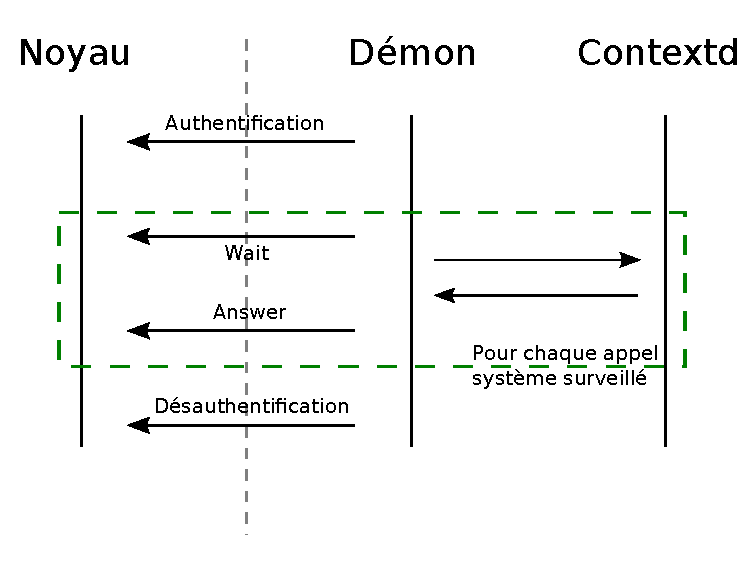
\includegraphics{global.pdf}
	\caption{Communication entre le noyau, le démon et contextd}
\end{figure}

%FIXME

Nous utilisons des mutex pour contrôler les échanges d'informations entre le noyau et le démon et assurer le traitement de chacun des appels système.
\begin{figure}[hb]
	\centering
	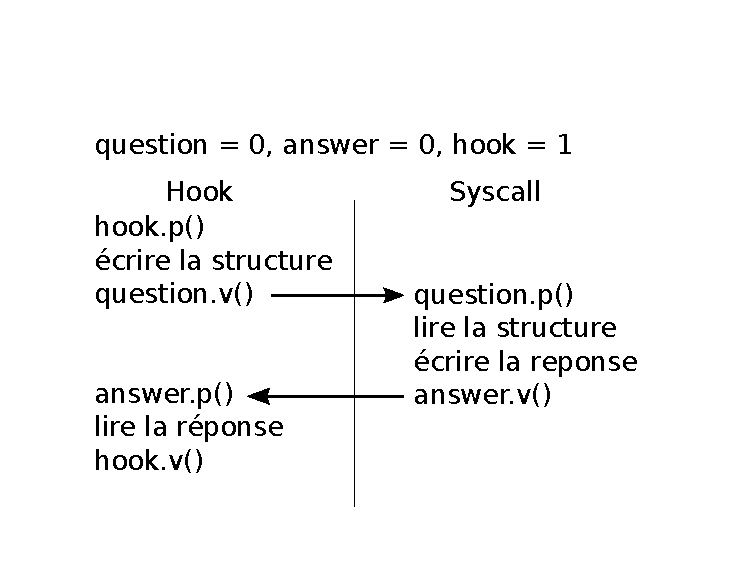
\includegraphics{syscall_sync.pdf}
	\caption{Communication entre les hooks LSM et les appels système}
\end{figure}

\subsubsection{L'interface présentée à l'administrateur}

	Pour faciliter l'administration et pour pouvoir intéragir plus aisément avec le noyau, nous avons mis en place deux "proc files" :
	
	\begin{itemize}
		\item /proc/contextd/programs : Ce fichier liste les programmes qui ont été enregistrés auprès du noyau et qui sont donc surveillés. Ce fichier n'est disponible qu'en lecture seule.
		\item /proc/contextd/status : Ce fichier est en revanche accessible en lecture/écriture. En lecture, il renvoie le PID de contextd (plus précisément le tgid (threads)). En ecriture, s'il reçoit un 0, il désactive la surveillance des programmes enregistrés et vide la liste.
	\end{itemize}


\subsection{Intéractions entre un processus, le noyau et contextd}

%FIXME Faire le schéma complet ...

\subsection{Ajouts à contextd}

Pour rendre contextd conscient de nos modifications nous avons implémenté plusieurs éléments :

%FIXME schéma des classes

Nous avons aussi rajouté un mécanisme permettant de nettoyer régulièrement la liste des clients enregistrés dans contextd, car cet action n'était pas présente.

De plus, notre solution nécessitant maintenant l'enregistrement des programmes auprès du noyau, il est désormé possible de charger dynamique cette liste de programmes à partir de /etc/context.d/program.d. Il est par contre nécessaire de préciser à contextd, à la compilation, les programmes à exclure de cette liste (pour l'instant firefox et claws-mail).

% Nous avons envisagé de créer trois nouveaux appels systèmes pour répondre au besoins de communications entre le noyau et contextd. Un appel système nous permet de renseigner et de transmettre une structure avec toutes les informations nécessaires à contextd. Cela nous évite ansi de parser du texte et facilite le processus d'authentification du démon qui correspond alors à un simple appel système lui aussi. La procédure d'authentification est une procédure séparée.
% 
% \begin{figure}[hb]
% 	\centering
% 	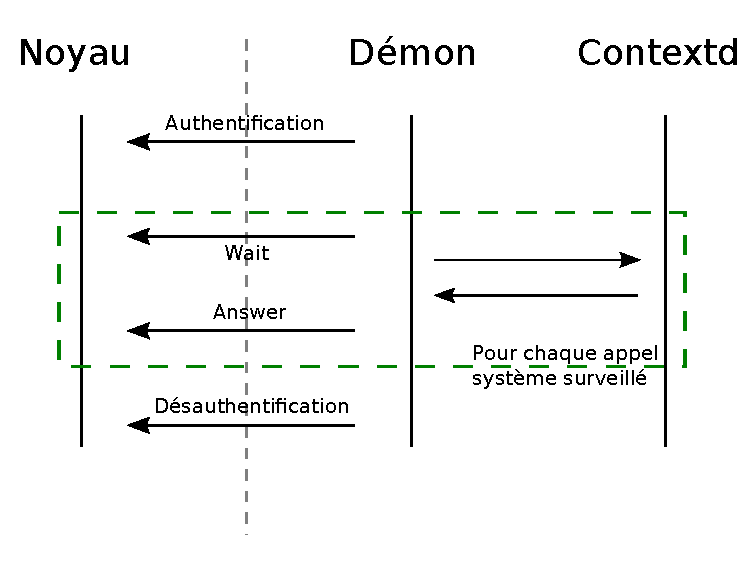
\includegraphics{global.pdf}
% 	\caption{Communication entre le noyau, le démon et contextd}
% \end{figure}
% %
% Il faut donc s'assurer que le démon se désauthentifie si le processus est terminé. \`A terme, ce comportement ne sera pas accepté.
% 
% Nous utilisons des mutex pour contrôler les échanges d'informations entre le noyau et le démon et assurer le traitement de chacun des appels système.
% 
% \begin{figure}[hb]
% 	\centering
% 	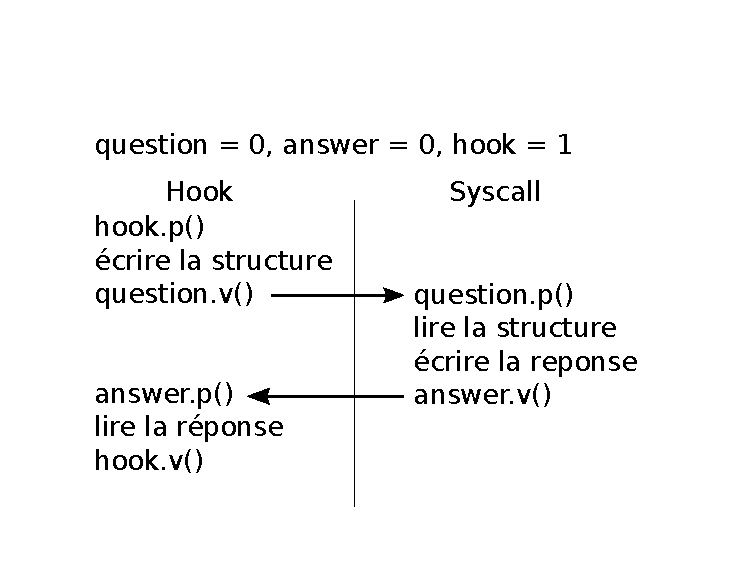
\includegraphics{syscall_sync.pdf}
% 	\caption{Communication entre les hooks LSM et les appels système}
% \end{figure}

NOTE : Nous partons du principe que notre travail est utilisé avec SELinux. Nous ne nous occupons pas de vérifier l'intégrité des programmes, intégrité préservée par SELinux.

Notre travail dépendant intégralement des solutions sous-jacentes.